\documentclass[12pt]{article}

\usepackage[letterpaper,hmargin=1.25in,vmargin=1.0in]{geometry}
\usepackage{bm} %bold math package: use command \bm{}
\usepackage{subfigure}
\usepackage{amsmath,amsfonts,amsthm,amssymb}
\usepackage{graphicx,psfrag}
\usepackage{nomencl}
\usepackage{verbatim}
%\usepackage{times,mathptm}
%\makenomenclature
%\makeglossary
%\topmargin      =-5.mm
%\oddsidemargin  =0.mm
%\evensidemargin =0.mm
%\headheight     =0.mm
%\headsep        =0.mm
%\textheight     =8.5in
%\textheight     =9.0in
\textwidth      =6.0in

\begin{comment}
%\renewcommand{\a}{\alpha}
%\renewcommand{\b}{\beta}
%\renewcommand{\d}{\delta}
\newcommand{\e}{\epsilon}
\newcommand{\f}{\phi}
\newcommand{\h}{\eta}
\newcommand{\g}{\gamma}
%\renewcommand{\l}{\lambda}
\newcommand{\m}{\mu}
\newcommand{\n}{\nu}
\newcommand{\q}{\theta}
%\renewcommand{\r}{\rho}
\newcommand{\s}{\sigma}
%\renewcommand{\t}{\tau}
\newcommand{\w}{\omega}
\newcommand{\y}{\psi}
\newcommand{\z}{\zeta}

\newcommand{\Y}{\Psi}
\newcommand{\F}{\Phi}
\newcommand{\W}{\Omega}
\end{comment}

\newcommand{\oo}{\infty}

\newcommand{\Dv}[1]{\frac{D #1}{D t}}
\newcommand{\dv}[2]{\frac{d #1}{d #2}}
\newcommand{\dvsq}[2]{\frac{d^2 #1}{d {#2}^2}}
\newcommand{\pd}[2]{\frac{\partial #1}{\partial #2}}
\newcommand{\pdc}[3]{\left(\frac{\partial #1}{\partial #2}\right)_{#3}}
\newcommand{\pdsq}[2]{\frac{\partial^2 #1}{\partial {#2}^2}}
\newcommand{\ave}[1]{\left\langle #1 \right\rangle}
\newcommand{\abs}[1]{\left\lvert #1 \right\rvert}
\newcommand{\del}{\nabla}
\newcommand{\cross}{\times}
\newcommand{\inner}[1]{\left\langle #1 \right\rangle}

\newcommand{\ba}{\mathbf{a}}
\newcommand{\bb}{\mathbf{b}}
\newcommand{\bc}{\mathbf{c}}
\newcommand{\be}{\mathbf{e}}
\newcommand{\br}{\mathbf{r}}
\newcommand{\bu}{\mathbf{u}}
\newcommand{\bx}{\mathbf{x}}
\newcommand{\by}{\mathbf{y}}
\newcommand{\bz}{\mathbf{z}}
\newcommand{\bA}{\mathbf{A}}
\newcommand{\bB}{\mathbf{B}}
\newcommand{\bF}{\mathbf{F}}
\newcommand{\bI}{\mathbf{I}}
\newcommand{\bR}{\mathbf{R}}
\newcommand{\bU}{\mathbf{U}}
\newcommand{\bV}{\mathbf{V}}

\newcommand{\ui}{\underline{i}}
\newcommand{\uk}{\underline{k}}

\newcommand{\tb}{\bar{t}}

\newcommand{\ft}{\tilde{f}}
\newcommand{\pt}{\tilde{p}}
\newcommand{\ut}{\tilde{u}}
\newcommand{\St}{\tilde{S}}

\newcommand{\bbR}{\mathbb{R}}

\newcommand{\sfe}{\mathsf{e}}
\newcommand{\sff}{\mathsf{f}}
\newcommand{\sfT}{\mathsf{T}}
\newcommand{\sfV}{\mathsf{V}}

\newcommand{\bgw}{\boldsymbol{\w}}
\newcommand{\gtb}{\bar{\t}}

\newcommand{\mvar}[1]{\mathit{#1}}
\newcommand{\subtx}[1]{\text{\it #1}}
\newcommand{\var}[1]{\text{\it #1}}

\newcommand{\sub}[1]{\textsf{#1}}
\newcommand{\file}[1]{\texttt{#1}}
\newcommand{\cfile}[2]{\texttt{#1}\textit{nnnn}\texttt{#2}}
\newcommand{\menu}[1]{\textsf{#1}}
\newcommand{\smenu}[2]{\textsf{#1$\to$#2}}
\newcommand{\ssmenu}[3]{\textsf{#1$\to$#2$\to$#3}}
\newcommand{\parm}[1]{\textit{#1}}
\newcommand{\dialog}[1]{\textsf{#1}}


\DeclareMathOperator{\tr}{tr}
\DeclareMathOperator{\Ren}{Re}

\newtheorem*{dfn}{Definition}
\newtheorem{problem}{Problem}

\numberwithin{equation}{section}


%%%%%%%%%%%%%%%%%%%%%%%%%%%%%%%%%%%%%%%%%%%%%%%%%%%%%%%%%%%%%%%%%%%%%%%%%%%%%%%%%%%%%
% PAGE HEADERS AND FOOTERS

% The geometry package lets set the margins.
% \usepackage[left=2cm,top=1cm,bottom=2cm,right=3cm]{geometry}

%\fancyhead[selectors]{output you want}

%The selectors are the following:E	even page
%O	odd page
%L	left side
%C	centered
%R	right side

\usepackage{fancyhdr} % Header and footer layout.
\pagestyle{fancy}

\fancyhf{} % Make header and footer empty, to be refilled below.

%\fancyhead[LE,RO]{Appendix 3}
%\fancyhead[LO,RE]{\thepage}
%\fancyhead[L]{Appendix 5}
\fancyhead[R]{\thepage}

% The layout of the header is to be completed yet.
%\lhead{Appendix 3}
%\rhead{\thepage}
%\fancyfoot[LE,RO]{\thepage} % Page numbers on the left on odd pages and on the right on even pages.
\renewcommand{\headrulewidth}{0pt} % Remove header line.
%\renewcommand{\footrulewidth}{0pt} % Remove footer line.
% \addtolength{\headheight}{0.5pt} % If not removed, make room for header line (e.g. if \headrulewidth is set to 0.5pt).

\fancypagestyle{plain}{% Redefine the plain page style (applied to the front page and the first pages of chapters).
\fancyhf{} % Make header and footer empty on plain pages.
%\fancyhead[LE,RO]{Appendix 3}
%\fancyhead[LO,RE]{\thepage}
%\fancyhead[L]{Appendix 5}
\fancyhead[R]{\thepage}

%\fancyfoot[LE,RO]{\thepage} % Page numbers on the left on odd pages and on the right on even pages.
%\renewcommand{\headrulewidth}{0pt} % Remove header line.
%\renewcommand{\footrulewidth}{0pt} % Remove footer line.
}

%%%%%%%%%%%%%%%%%%%%%%%%%%%%%%%%%%%%%%%%%%%%%%%%%%%%%%%%%%%%%%%%%%%%%%%%%%%%%%%%%%%%%

\setcounter{page}{1}
%\title{\bf Description of Automatic Simulation Cycling Options
%             Between Combustion and Melt Spaces}
%\begin{flushleft}
%\bf{Appendix 3}
%\end{flushleft}

\title{  \bf GFM 4.0 Automatic Cycling Guide}
%\date{\today}
%\author{S.A.~Lottes}
\date{}
\begin{document}
\maketitle
%========================================================================
\section{Introduction to Cycling}
\label{sec:intro}
%========================================================================
Automatic simulation cycling between combustion and melt spaces is a process implemented in the graphical user interface (GUI) and control program of the \emph{Glass Furnace Model} (GFM) that allows a coupled solution of conditions in the combustion and melt domains to be achieved with minimal user intervention. The cycling includes exchange of the common boundary information at the melt surface. This feature allows a large number of cycles to be carried out without the user having to copy melt surface boundary condition files between directories or having to manually start up the computation again in the domain that comes next in a long sequence of cycles. Essentially all of this can be accomplished in an unattended run in the domain cycling mode of operation. With this feature the intervals for exchange of the common melt surface boundary information can be shortened (because no human intervention is required) providing more frequent exchange of information between spaces and therefore tighter coupling. Automatic domain cycling can be set for both regular and regenerative furnace simulations.
This document describes the domain cycling feature and how to set up and initiate automatic domain cycling runs in the graphical user interface and control program.\\
\\
Four new menu choices have been added to the main \menu{Simulation} menu to start up automatic domain cycling runs.   
These new \menu{Simulation} sub-items are:
\begin{itemize}
\item[ ] \menu{Cycle Domains (Comb First)}
\item[ ] \menu{Cycle Domains (Melt First)}
\item[ ] \menu{Cycle Regenerative (Comb First)}
\item[ ] \menu{Cycle Regenerative (Melt First)}
\end{itemize}
Selecting one of these menu items pops up a \dialog{Provide Cycle Information} dialog box, shown in Figure~\ref{PCI-dialog}, asking for the number of cycles to run, and allowing the user to change the maximum number of computation iterations to perform for the major stages of the cycle. In addition, if the option to scale the heat flux into the melt is on, the number of cycles to continue scaling may be specified. This mode of running provides a way to approach an expected solution before turning scaling off. If fuel flow in the combustion space has been set to provide sufficient energy to the melt to reach a known glass outlet temperature, scaling ensures that required energy enters the melt during early cycles when temperatures have not yet approached a stable mean in both spaces. Note that if the option to scale the heat flux into the melt is off, then the number of cycles to continue scaling entered in the dialog box is ignored.\\

\begin{figure}
\centering
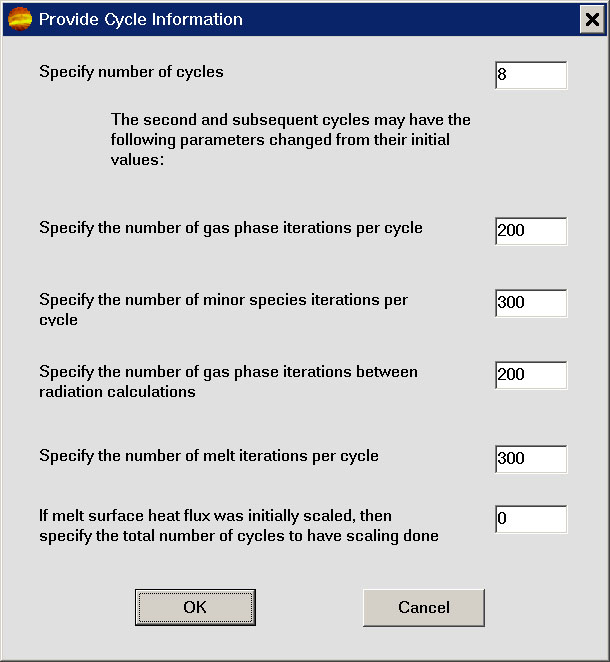
\includegraphics{figs/cycleBox.jpg}
\caption{Provide Cycle Information Dialog Box}
\label{PCI-dialog}
\end{figure}
%\\
\noindent
After \parm{OK} is entered for the \dialog{Provide Cycle Information} dialog box, the \dialog{Select Existing Case to Simulate} dialog box appears and allows the user to navigate through the file system to the file folder of the case to simulate. If the melt space simulation is to be run first, the simulation must be started from the case folder in the melt directory. If the combustion space simulation is to be run first, the simulation must be started from the case folder in the combustion directory. The case must be set up for automatic cycling in both the melt and combustion space case definitions as described in the following sections.\\
\\
Coupling between the combustion and melt spaces is accomplished by passing the heat flux, both radiation and convection, to the melt surface calculated in the combustion domain to the melt domain and then passing the surface temperature calculated in the melt domain to the combustion domain automatically. The user interface and control program copies the appropriate melt surface temperature and heat flux distribution files back and forth between the melt and combustion subdirectories. The melt and combustion spaces are coupled through the energy equation boundary conditions at the melt surface. In the combustion space, the surface temperature computed in the melt code is the boundary condition. In the melt space, the surface heat flux distribution computed in the combustion space code is the boundary condition. Tight coupling between the two spaces requires that these conditions be swapped frequently. Automatic cycling allows this swapping to be done many times in an unattended overnight or over-weekend run. The iteration limits set in the \dialog{Provide Cycle Information} dialog box control the swap points and swap frequency.

%========================================================================
\section{Cycle Domains Algorithm}
\label{sec:cda}
%========================================================================

The algorithm for automatic cycling of domains with the combustion space run first is as follows:

\noindent
\begin{enumerate}
	\item Clicking on the \smenu{Simulation}{Cycle Domains (Comb First)} menu item will begin a regular combustion simulation for a four digit case number ``\textit{nnnn}'' determined by the \cfile{case}{} folder chosen.
	\item When the combustion simulation stops, a melt simulation is automatically started for the same case number using the heat flux data from the combustion domain.
	\item  When the melt simulation stops, one cycle is complete.
	\item  The combustion simulation is automatically restarted using the surface temperature distribution data from the melt domain and it runs until it completes (a user specified number of iterations).
	\item  The melt simulation is automatically restarted after the combustion simulation completes.
	\item  The whole cycling process (repeating steps 4 and 5) stops when a specified number of cycles has been completed.
\end{enumerate}

\noindent
The active domain, combustion or melt, and the cycle number are shown in a light blue box in the lower right corner of the main GFM window when in simulation mode. The display switches between the combustion and melt space depending on which is active.\\ 
\\
The mean relative change in coupling conditions, heat flux distribution and temperature distribution at the melt surface can be checked to determine if a coupled simulation is sufficiently converged. If not, another set of cycles can be run. The mean relative change in coupling conditions can also be displayed as a dynamically updated plot on-screen (Refer to the RunPlot documentation), and the cycling can be terminated when the mean relative change is sufficiently small.\\
\\ 
The algorithm for automatic cycling of domains with the melt space first is the same as that for doing the combustion space first, enumerated above, except that the melt computation is run first. Both spaces can be sensitive to the boundary conditions at the surface that they share, and consequently convergence of the coupled solution may depend on how close the initial guess or starting point is to a converged solution. Because energy requirements for the melt space can be estimated from batch feed rates and material properties based on a reasonably close estimate of the melt exit temperature, a melt space computation done first with scaling turned on may give a surface temperature distribution that is a good estimate for a first combustion space computation, if the average melt temperature has begun to approach its asymptotic value.\\
\\
If cycling with the melt computation done first does not converge, cycling with the combustion space run first with a uniform surface temperature based on a good estimate of expected mean surface temperature may succeed. The melt surface temperature is the primary known surface temperature boundary used in the radiation enclosure exchange calculation. Wall surfaces use a known heat flux boundary condition in this computation based on a heat balance at the wall that includes incoming radiation from the emitting media. Consequently, wall temperatures tend to approach temperatures that are slightly above the melt surface temperature (just enough higher to re-radiate the additional amount arriving from the flame minus the amount lost through the walls). 

%========================================================================
\section{Setup for Cycle Domains}
\label{sec:setup}
%========================================================================

Various strategies can be used to prepare for automatic cycling:
\noindent
\begin{enumerate}
	\item[A.] The simplest strategy is to set up initial conditions the same as the subsequent cycle conditions. However, this strategy may require a very large number of cycles to be run before convergence is achieved.
	\item[B.] If desired, both or either one of the domains may be simulated for a while independently and later restarted for the cycling process. Before doing an automatic cycling run this strategy could be used to verify that iterating in each domain was possible or it could be used to establish a basic flow field in each domain and approach a stable mean temperature. This strategy could reduce the number of cycles required for convergence, but manual intervention is needed before the automatic cycling is started.
	\item[C.] A combination strategy is to set up the initial cycle conditions to iterate long enough to establish a flow field and approach a stable mean temperature. The number of iterations in the subsequent cycles is greatly reduced to provide frequent swapping of surface boundary condition data. This strategy could also reduce the number of cycles required for convergence. Strategy C is described here.
\end{enumerate} 

\noindent
Setting up a combustion first automatic cycling of domains simulation consists of the following: 

\noindent
\begin{enumerate}
	\item Create a combustion case and a melt case with the same case number. The bottom dimensions of the combustion domain should match the top dimensions of the main melt surface component (excluding refiner area) in the melt domain.
	\begin{itemize}
		\item During the initial case definition, set these necessary combustion parameters:
		\begin{itemize}
			\item While in the preprocessor combustion domain, click on the\\ \smenu{Properties}{Simulation Parameters} menu item to display 4 lists of parameters in green boxes.
			\item Click on the second item in the first (leftmost) green box until parameter \parm{new start} is displayed and then set the \parm{initial iterations} (fourth line in the rightmost green box) to a number that will allow an initial flow field to be established, 600 appears to be reasonable. (For strategy B the parameter will be \parm{restart}. For strategy A and B the \parm{initial iterations} would likely be from 100 to 200.)
			\item Set the combustion parameters to indicate that radiation will be calculated. Click on the bottom item in the leftmost green box until parameter \parm{calc radiation} is displayed. 
			\item The radiation \parm{interval} (displayed in the bottom item of the third green box) must not be greater than the number of gas phase \parm{iterations} (displayed in the third item in the first green box). \parm{interval} is the number of combustion space fluid dynamic iterations between radiation computations that include absorbing and emitting media and the wall and melt surface enclosure radiation exchange computation. Immediately after a radiation computation an updated set of melt surface heat flux distribution values is available.
			\item For automatic cycling, the \parm{iterations} parameter should be set equal to \parm{interval}. This will cause the updated melt surface heat flux set to be transferred to the melt computation as soon as it is available. The default for these values is 200 in the combustion space. More experience is needed to determine what value is optimum. Any feedback on user experience would be appreciated.
			\item (For a combustion space only run the \parm{iterations} parameter should be about 6 to 8 times the \parm{interval} value.)
			\item Set the melt surface temperature type (in the first item of the fourth green box). If the melt domain has already been simulated, then the surface type can be set to indicate that the melt simulation has calculated the temperature (\parm{melt surf: calculated}). Otherwise indicate that the temperature is specified (\parm{melt surf: specified}) and set the initial surface temperature in the next item of the fourth green box. After the first cycle, the control program will set parameters so that the melt surface temperature in the combustion space will be the distribution calculated from the melt domain.
			\end{itemize}
		\item During the initial case definition, set these necessary melt parameters:
		\begin{itemize}
			\item While in the preprocessor melt domain, click on the \smenu{Properties}{Simulation Parameters} menu item to display 3 lists of parameters in green boxes.
			\item Click on the second item in the first (leftmost) green box until parameter \parm{new start} is displayed. (For strategy B the parameter will be \parm{restart}). 
			\item The melt simulation will be done after a combustion simulation so the heat flux will be determined by the combustion calculation. Set the melt heat flux parameter to indicate either \parm{heat flux: fixed} or \parm{heat flux: scaled} with the next line showing \parm{calc. in combustion}. Click on the second item in the third green box until the desired option is displayed.
			\item The \parm{heat flux: scaled} parameter indicates that the combustion calculated surface heat flux will be scaled to meet heat requirements needed to reach a user specified liquid glass exit temperature. This heat requirement calculation for scaling includes heat needed for solids heating, solids melting, liquid glass heating, melt tank wall losses, and the heat added by electric boosters.
			\item In automatic cycling mode the \parm{iterations} parameter in the melt is the number of global solver iterations that will be performed before switching back to the combustion space. Because the melt is essentially a large reservoir it tends to respond rather slowly to changing conditions, such as an updated heat flux from the combustion space. Several thousand total iterations in the melt may be required to reach a converged steady state melt solution. Therefore, the \parm{iterations} could initially be set to a large number, 3000 appears to be reasonable.
(For strategy A and B, setting \parm{iterations} in the melt to a value between 200 and 400 appears reasonable.)   					\end{itemize}   
	\end{itemize}
	\item After saving both the combustion and melt cases in the preprocessor, go back to the main menu
and click on the \smenu{Simulation}{Cycle Domains (Comb First)}, to bring up the \dialog{Provide Cycle Information} dialog box with default values. Enter the number of cycles to run in this set of automatic cycles if the desired number is different from the default. The GFM control program keeps track of the number of cycles in the current set of cycles. If an additional set of cycles is activated, the simulations will continue where they had left off previously, but the cycle count itself will begin anew. In other words, the GFM control program does not keep track of a global cycle count; each set of cycles starts with cycle number 1.  
	\item Whereas the parameters specified during the initial case definition apply to the first cycle in the set of cycles to be done, the remaining information provided on the \dialog{Provide Cycle Information} dialog box apply to the second and subsequent cycles in the set. Changing both the number of gas phase iterations per cycle and the number of gas phase iterations between radiation calculations to 100 may speed up convergence by swapping heat flux in shorter intervals than the default 200, however, the radiation computation takes a long time, and therefore, doing it before the flow field has begun to stabilize in the new cycle may lead to longer convergence times. Some experimentation and watching convergence rates of the mean temperatures and equation residuals with the \sub{RunPlot} program may be necessary to optimize iteration count settings. 
	\item Note that the last entry in the dialog box is ignored when scaling has not be specified for the melt surface heat flux. Also, the ``total number of cycles'' mentioned for this entry applies to the number of cycles for the current cycle set.  
	\item After clicking the \parm{OK} button on the \dialog{Provide Cycle Information} dialog box, select the case to cycle from the \dialog{Select Existing Case to Simulate} dialog box and click the \parm{Simulate} button to start the cycling.
	\item Note that the user may stop the cycling run gracefully during any cycle by clicking on the \menu{Stop Run} menu item and indicating that the run should stop after the current cycle has completed.
\end{enumerate}

\noindent
Setup for a melt first automatic cycling of domains is similar to the setup for combustion first, except for the melt surface conditions. In the melt domain set the \parm{heat flux: fixed} or \parm{heat flux: scaled} parameter with the next line showing \parm{uniform value} and provide that value on the following line. In the combustion domain set the first line in the rightmost green box to be \parm{melt surf: calculated}. Also, the menu item to begin automatic cycling will be \smenu{Simulation}{Cycle Domains (Melt First)}.

%========================================================================
\section{Alternatives After Running an Automatic Cycle Set}
\label{sec:altern}
%========================================================================
\noindent
The status of a case after automatic cycling is different from the status of a case after running a regular simulation. When the user saves a case in the preprocessor, an input file to the CFD code is created from the user's definition of the case. After running a regular simulation that input file is still in sync with the case definition. However, the GFM control program modifies the CFD code input files during automatic cycling, but does not modify the case definition. Therefore, determining what to do after an automatic cycling run must account for the differences in case status.\\
\\
After running an automatic cycle set and evaluating the results, the user may choose to proceed in a variety of ways. The primary options are described below.
\begin{itemize}
	\item \textbf{Start Over:} If the run results look bad, then the user may decide to start over from scratch with different parameter and control settings. The best way to start over is to get into the \ssmenu{Pre-Processor}{Combustion Space or Glass Melter}{File} menu and click on \menu{Delete Case Results}. Then the user can open up the case in the preprocessor, change the case definition as needed, and proceed from that point with a new start.
	\item \textbf{Continue cycling with another cycle set:} If a review of results indicates that more cycles are needed to reach a stable converged solution, another automatic cycling run can be started and it will pick up where it left off as long as no changes are made to the case via the user interface that result in the user saving a changed case. To simply run another cycle set from the state where the last one finished, the user should go back to the main menu, click on the same \smenu{Simulation}{Cycle Domains ...} that was used before, and enter the appropriate information in the \dialog{Provide Cycle Information} dialog box. 
	\item  \textbf{Continue cycling with changed parameters:} If an automatic cycling run is to be restarted with changes to operating parameters via the user interface that require saving the case, then the following run parameters must also be set to restart an automatic cycling run. These steps bring the case definition files into sync with the run setup files passed to the combustion and melt CFD codes during cycling. (Note that automatic cycling cannot be restarted if either of the grids are modified.)
 
For the combustion space case, with the case open:
	\begin{enumerate}
	    \item Display the green simulation parameters boxes by clicking on the\\ \smenu{Properties}{Simulation Parameters} menu item.
	    \item If the first parameter under \parm{Parameters} in the first green box indicates \parm{new start}, click it so that it indicates \parm{restart}.
	    \item Set the surface temperature type (in the first item of the fourth green box) to indicate that the melt simulation has calculated the temperature (\parm{melt surf: calculated}).
	\end{enumerate}

For the melt space case, with the case open:
	\begin{enumerate}
	    \item Display the green simulation parameters boxes by clicking on the\\ \smenu{Properties}{Simulation Parameters} menu item.
	    \item If the first parameter under \parm{Parameters} in the first green box indicates \parm{new start}, click it so that it indicates \parm{restart}.
	    \item Set the \parm{iterations} to the value used for number of melt iterations set in the \dialog{Provide Cycle Information} dialog box used for subsequent cycles from the previous cycle set (default 300). This parameter should be set larger if an operating condition has been changed that would significantly change the mean temperature of the melt.
	    \item Set the melt heat flux parameter to indicate either \parm{heat flux: fixed} or \parm{heat flux: scaled} with the next line showing \parm{calc. in combustion}. 
	 \end{enumerate}

\item \textbf{Start a new case cycling with changed parameters from the state of a converged case:} If the run results look good and converged, then the user may decide to use this case as a base for other cases, for example to do parametric studies. Get into the \ssmenu{Pre-Processor}{Combustion Space or Glass Melter}{File} menu and open the case. Then return to the same menu and click on \menu{Save Case As (Full case)} to make a copy of the case using a new case number. Make operational parameter changes as desired in the new case and proceed as indicated in the previous bullet item above. 

\item \textbf{Stop:} If the run results look good and converged, then the user may decide to do nothing more with the case. 

\end{itemize}


%========================================================================
\section{Regenerative Furnace Cycle Algorithm}
\label{sec:regen}
%========================================================================
\noindent
\begin{itemize}
\item The regenerative furnace cycle algorithm builds upon the cycle domain algorithm.
\item Domain cycling for regenerative furnaces is started via a \smenu{Simulation}{Cycle~Regenerative} item from the main menu.
\item  For a regenerative furnace simulation, two combustion space domain simulations are done, one for each of the burner and exhaust firing patterns. The setup for these simulations of alternate firing patterns is described in the next section.
\item  Both combustion domain simulations pass a melt surface heat flux distribution to the melt domain simulation and the two sets of data are averaged together for use. The melt domain will pass surface temperature data to both of the combustion domain simulations for the next cycle.
\end{itemize}

\noindent
This algorithm for simulation of regenerative furnaces assumes that the melt acts as a large heat reservoir and responds slowly to the alternating changes in firing pattern of the regenerative furnace. The asymptotic state of the melt for a single firing pattern may be simulated by setting up a case with the desired firing pattern and running it as a non-regenerative furnace case.
\newpage
%========================================================================
\section{Setup for Regenerative Furnace Domain Cycling}
\label{sec:regen-setup}
%========================================================================
\noindent
\begin{itemize}
\item Construct burners and exhausts as usual for one of the two firing patterns in the combustion space grid. Set other parameters as needed for this firing pattern. Save the setup using a case number, $N$, where the next consecutive case number $N+1$ is not in use.
\item  The case number for the $2^{nd}$ burner firing pattern must be $N+1$. A starting point for creating the $N+1$ case with the alternate firing pattern may be created by using the \smenu{File}{Save Case As} menu item to save combustion case $N$ as case $N+1$.
\item  Modify the furnace figure for case $N+1$ so that the exhausts become burners and burners become exhausts to create the second, alternative firing configuration for the
regenerative furnace, or do whatever is needed to define the $2^{nd}$ burner firing configuration.

 For example, for a furnace with one burner, $B1$, and one exhaust, $E1$:
	\begin{enumerate}
	\item Add exhaust $E2$ and set its position to be centered over burner $B1$.
	\item Add burner $B2$ and set its position to be centered over exhaust $E1$.
	\item Delete $B1$
	\item Delete $E1$
	\end{enumerate}
\item  Make adjustments to other flow parameters as needed to match the furnace operating conditions in the alternate burner firing mode.
\item  Set up the melt space as usual using case number $N$. Do not set up a melt space for case number $N+1$.
\item  When all is ready, start an automatic cycling simulation by selecting menu item \\ \smenu{Simulation}{Cycle~Regenerative}.
\end{itemize}

\end{document}

